\documentclass[border={5pt 0pt 20pt 5pt}, preview]{standalone}

\usepackage{pgfplots}
\pgfplotsset{compat=1.15}
\usepackage{xcolor}


\usepackage{tikz}
\usepackage[utf8]{inputenc}
\usepackage{xfp}
\usepackage{booktabs}
\usetikzlibrary{calc}
\usepackage{graphicx}

\newcommand{\Del}[1]{\textit{$\Delta$\MakeLowercase{#1}}}
\newcommand\ratio[2]{%
    \pgfmathparse{ #1/(#1 + #2)}\pgfmathresult
}


\newcommand\colorBar{
    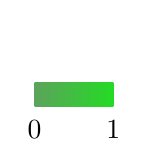
\begin{tikzpicture}[baseline={(0,0)}, inner sep=0,outer sep=0]

       
        \pgfdeclarehorizontalshading{someShading}{4cm}{
        color(0cm)=(green!0!gray);
        color(4cm)=(green!100!gray)
        }
        
        \shade [shading=someShading, yshift=-1cm]  (0,0) rectangle ++(1,0.3);
        \node [] at (0,-1.3) {0};
        \node [] at (1,-1.3) {1};
        
        \end{tikzpicture}
}


\newcommand\particle[2]{%
  \begin{tikzpicture}[x=2cm, y=2cm]
  

  % Calculate the ratio of nucleus to cytosol concentration
  \def\nratio{\fpeval{ round(#1/(#1 + #2),2)}  };
  \def\cratio{\fpeval{ round(#2/(#1 + #2),2)}  };

  \def\nconc{\fpeval{ round(#1,1)}  };
  \def\cconc{\fpeval{ round(#2,1)}  };
  
  %Node for Circles
  \node at (0,0) [circle,draw, scale=1 ,fill=green!\fpeval{round(100*(\cratio))}!gray] (c2) {};
  
  \node at (0,0) [circle,draw, scale=0.5 ,fill=green!\fpeval{round(100*(\nratio))}!gray] (c1) {};
  
  
  %Node for line ends
  \node [inner sep=0,outer sep=0, xshift=0.2cm] at (c1.east) (n_conc) {};
  \node [inner sep=0,outer sep=0,yshift = -0.09cm] at (n_conc.south) (c_conc) {};
  
  % Node for data
  \node [inner sep=0,outer sep=0, xshift=0.cm, text width = 0cm, align=left] at (n_conc.east) {\scalebox{.2}{\nconc} };

  \node [inner sep=0,outer sep=0, xshift=0.cm, text width = 0cm, align=left] at (c_conc.east) {\scalebox{.2}{\cconc}};
  
  % Draw Lines
  \draw[-, very thin] (n_conc) -- (c1);
  \draw[-, very thin] (c_conc) -- (0.16cm,-0.1065cm);

  
  \end{tikzpicture}
}

\newcommand\cell[2]{
    \begin{tikzpicture}[baseline={(c_conc.base)}, x=2cm, y=2cm, , outer sep=0]
  
        %Node for Circles
        \node at (0,0) [circle,draw, scale=1] (c2) {};
        
        \node at (0,0) [circle,draw, scale=0.5] (c1) {};
        
        
        %Node for line ends
        \node [inner sep=0,outer sep=0, xshift=0.2cm] at (c1.east) (n_conc) {};
        \node [inner sep=0,outer sep=0,yshift = -0.09cm] at (n_conc.south) (c_conc) {};
        
        % Node for data
        \node [inner sep=0,outer sep=0, xshift=0.cm, text width = 0cm, align=left] at (n_conc.east) {\scalebox{.2}{#1} };
        \node [inner sep=0,outer sep=0, xshift=0.cm, text width = 0cm, align=left] at (c_conc.east) {\scalebox{.2}{#2}};
        
        % Draw Lines
        \draw[-, very thin] (n_conc) -- (c1);

        \draw[-, very thin] (c_conc) -- (0.16cm,-0.1065cm);

        \end{tikzpicture}
    
}

\newcommand\drawcell[2]{%
    \begin{tikzpicture}[baseline={(c_conc.base)}, outer sep=0]
        \def\sc{3}
        \node at (0,0) [scale=\sc] {\cell{#1}{#2}};
    \end{tikzpicture}
}

\newcommand\drawRatio[2]{%
    \begin{tikzpicture}[baseline={(c_conc.base)}, outer sep=0]
        \def\sc{3}
        \node at (0,0) [scale=\sc] {\particle{#1}{#2}};
    \end{tikzpicture}
}



\begin{document}

\begin{tabular}[c]{p{1.4cm}p{1.8cm}p{2.8cm}|p{1.8cm}p{1.6cm}}
    \toprule
    \multicolumn{1}{c}{} & \multicolumn{2}{c}{\textbf{Healthy Mitochondria}} & \multicolumn{2}{c}{\textbf{Damaged Mitochondria}} \\ \midrule
     &\textbf{Simulation} & \multicolumn{1}{c}{\textbf{Data}}\hspace{0.52cm}  & \textbf{Simulation} & \hspace{0.5cm}\textbf{Data}  \\ 
     &   \multicolumn{4}{c}{\textbf{Rtg3-GFP}}  \\
    WT & \drawRatio{215.7662572994662}{193.73735468865948} & \drawRatio{0}{1} & \drawRatio{346.2757699180584}{63.22784207023777} & \drawRatio{1}{0} \\
    \Del{Rtg1} & \drawRatio{366.1582049113594}{43.34580707693283} & \drawRatio{1}{0}  & \drawRatio{366.1589600110554}{43.34505197723719} & \drawRatio{1}{0} \\
    \Del{Rtg2} & \drawRatio{215.76640011596893}{193.737211869589} & \drawRatio{0}{1}& \drawRatio{215.76640470566127}{193.73720728246383} & \drawRatio{0}{1} \\
    \Del{Mks} & \drawRatio{347.64927120440973}{61.85434078386726} & \drawRatio{1}{0}& \multicolumn{2}{r}{}  \\
    \Del{Rtg2}\Del{Mks} & \drawRatio{347.64927315432374}{43.34580707693283} & \drawRatio{1}{0} & \multicolumn{2}{r}{} \\ 
     &   \multicolumn{4}{c}{\textbf{Rtg1-GFP}}   \\
    WT & \drawRatio{54.89009874232648}{91.03025761443399} & \drawRatio{0}{1} & \drawRatio{110.37166243874616}{35.54869391809153} & \drawRatio{1}{0} \\
    \Del{Rtg3} & \drawRatio{0.07820900778318428}{145.842547349088} & \drawRatio{0}{1}& \drawRatio{0.07845351771792033}{145.84230283909895} & \drawRatio{0}{1} \\
    \Del{Rtg2} & \drawRatio{54.890193652195336}{91.03016269915003} & \drawRatio{0}{1} & \drawRatio{54.89019658629695}{91.0301597704889} & \drawRatio{0}{1} \\ 
    \Del{Mks} & \drawRatio{111.06393160920344}{34.856424747619194} & \drawRatio{1}{0}& \multicolumn{2}{r}{}  \\
    \Del{Rtg2}\Del{Mks} & \drawRatio{111.06393280959674}{34.856423547230804} & \drawRatio{1}{0} & \multicolumn{2}{r}{} \\ 
      &   \multicolumn{4}{c}{\textbf{Rtg2-GFP}}   \\
    WT & \drawRatio{0}{651.6543766184084} & \drawRatio{0}{1} & \drawRatio{0}{651.6543766184084} & \drawRatio{0}{1} \\
    &  \multicolumn{4}{c}{
        
    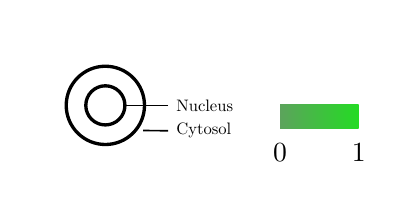
\begin{tikzpicture}
        \node [] (cell) {\drawcell{Nucleus}{Cytosol}};
        \node [ right of=cell, xshift=1.5cm] (col) {\colorBar};
    \end{tikzpicture}
    } 
    
    \\
    \bottomrule
\end{tabular}

\end{document}
